% \begin{document}
\chapter{Approximation Algorithms}
\section{When Relaxing Integrality is Not for Free: Approximation Algorithms}

Thousands (or millions :)) of optimization problems have been proved to be NP-hard, which means
that finding optimal solutions for them is very likely to be intractable. More specifically, unless
$\mathsf{P}=\mathsf{NP}$, there is no algorithm for an NP-hard optimization problem that satisfies
all of the following three desiderata:
\begin{enumerate}
  \item The algorithm is \emph{efficient} (runs in polynomial time).
  \item The algorithm is \emph{reliable} (works for any input instance).
  \item The algorithm finds an optimal solution (\emph{optimality}).
\end{enumerate}
Therefore, when confronted which such problems, we need to relax one of the above conditions when
dealing with NP-hard optimization problems. If we relax reliability, then we get \emph{heuristics}
that are designed to work well on instances that commonly appear in practice. If we relax the third
condition, we obtain \emph{approximation algorithms}. The notion of approximation algorithms allows
us to obtain a more fine-grained picture of the difficulty of NP-hard optimization problems: some
problems turn out to have very good approximations, whereas others resist such attempts.

The formal definition of approximation algorithms is as follows.

\dfn{$ \alpha $-approximation algorithm}{
An $\alpha$-approximation algorithm for a given optimization problem is an algorithm that runs in
polynomial time and outputs a solution $S$ such that:
\begin{itemize}
  \item $\dfrac{\mathrm{cost}(S)}{\mathrm{cost}(\text{Optimal solution})}\le\alpha$ if the problem is
    a minimization problem,
  \item $\dfrac{\mathrm{profit}(S)}{\mathrm{profit}(\text{Optimal solution})}\ge\alpha$ if the
    problem is a maximization problem.
\end{itemize}
}

It is clear that we will have $\alpha\ge 1$ for minimization problems and $\alpha\le 1$ for
maximization problems. Moreover, if $\alpha=1$, then we have an efficient exact algorithm (and the
problem is in $\mathsf{P}$). The goal when designing approximation algorithms is to achieve a
guarantee $\alpha$ that is as close to $1$ as possible. We now introduce a general framework for
using linear programming in the design of approximation algorithms followed by an application:
vertex cover.

\section{Using Linear Programming to Design Approximation Algorithms}

Consider a minimization problem. When considering the definition of approximation algorithms, it
seems very hard, even for a specific instance of the problem, to analyze the approximation guarantee
$\frac{\mathrm{cost}(S)}{\mathrm{cost}(\text{Optimal solution})}$ of the algorithm on the instance,
as we are comparing ourselves with an optimal solution (that is most likely very hard to compute and
does not possess any nice structure). The solution to this is to compare ourselves with a lower bound
on the optimum. Indeed, we then have that
\[
  \frac{\mathrm{cost}(S)}{\mathrm{cost}(\text{Optimal solution})}
  \ \le\ \frac{\mathrm{cost}(S)}{\text{lower bound on opt}}\ \le\ \alpha.
\]
From the above, it is clear that we need a good lower bound to be able to claim a good guarantee
$\alpha$. To obtain such a lower bound (and to design the approximation algorithm), linear
programming is super handy. A popular framework is as follows:
\begin{enumerate}
  \item Give an exact formulation of the problem as Integer LP -- usually with binary variables
    ($x_i\in\{0,1\}$).
  \item Relax to LP -- $x_i\in[0,1]$
\end{enumerate}

\begin{center}
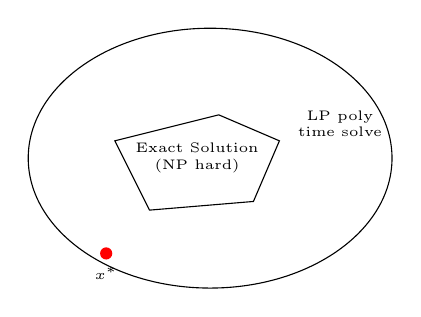
\begin{tikzpicture}[scale=1.1]
  \draw (0,0) ellipse (2.1cm and 1.5cm);
  \draw (-1.1,0.2) -- (0.1,0.5) -- (0.8,0.2) -- (0.5,-0.5) -- (-0.7,-0.6) -- cycle;
  \node[font=\tiny,align=center] at (-0.15,0) {Exact Solution\\(NP hard)};
  \node[font=\tiny,align=center] at (1.5,0.4) {LP poly\\time solve};
  \fill[red] (-1.2,-1.1) circle (2pt);
  \node[font=\tiny,below] at (-1.2,-1.15) {$x^*$};
\end{tikzpicture}
\end{center}

\begin{enumerate}[resume]
  \item Solve LP to get a optimal solution $x^*$ to the LP which is a lower (upper) bound on the
    optimal solution to Integer LP and thus the original problem. Then somehow round $x^*$ to an
    integral solution ``without losing too much'' (which will determine the guarantee $\alpha$).
\end{enumerate}

We now use the above framework for the vertex cover problem, and then introduce the concept of
\emph{integrality gap}.

\subsection{Vertex Cover}

Here, we apply the framework to get an approximation algorithm for the \emph{Vertex Cover} problem.
First recall the definition:

\dfn{Vertex Cover (VC) Problem}{
Given a graph $G=(V,E)$ and a weight function on the vertices $w:V\to\mathbb{R}_+$, output a set
$C\subseteq V$ of minimum weight such that for all $\{u,v\}\in E$, $u\in C$ or $v\in C$.
}

First, we define an ILP solving VC: For all $v\in V$, we introduce a variable $x_v$, which is $1$
if $v\in C$, and $0$ otherwise. The objective function is
\[
  \min\sum_{v\in V}w(v)x_v
\]
and for each $\{u,v\}\in E$ we introduce the constraint $x_u+x_v\ge 1$. This ensures that for each
edge, at least one endpoint is in $C$. Additionally, we require that for each $v\in V$ we have
$x_v\in\{0,1\}$. Note that at this point our Integer LP formulation is exactly equivalent to the
original problem.

Second, we relax the ILP to an LP by allowing that $x_v\in[0,1]$. Actually, it's sufficient to
require that $x_v\ge 0$, because having an $x_v$ greater than $1$ will not satisfy any additional
constraint, but only increase the value of the objective function, so this will not happen in an
optimal solution.

Third, we have to do the rounding: Suppose we've solved the LP and got an optimal solution $x^*$.
We will return $C=\{v\in V: x^*_v\ge\frac12\}$ as our solution to VC.

\clm{}{}{
$C$ is a feasible solution.
}

\pf{}{
Consider any edge $\{u,v\}$ and its constraint. Since $x^*_u+x^*_v\ge 1$, at least one of
$x^*_u,x^*_v$ is $\ge\frac12$ and thus in $C$.
}

\clm{}{}{
The weight of $C$ is at most twice the value of the optimal solution of VC.
}

\pf{}{
We have
\[
  \sum_{v\in C}w(v)=\sum_{v\in V:\,x^*_v\ge\frac12}w(v)\ \le\ \sum_{v\in V:\,x^*_v\ge\frac12}2x^*_v w(v)
  \ \le\ \sum_{v\in V}2x^*_v w(v)=2\sum_{v\in V}x^*_v w(v)=2\LPOPT\le 2\VCOPT
\]
where the first inequality holds because $2x^*_v\ge 1$.
}

So, we have designed a $2$-approximation algorithm for Vertex Cover. This is a simple algorithm
using linear programming. To appreciate the power of the framework, I challenge you to find a
$2$-approximation algorithm for Vertex Cover (with node-weights) without the use of LPs. (It is
possible but quite difficult.)

\subsection{Integrality Gap}

The notion of the \emph{integrality gap} allows us to bound the power of our linear programming
relaxation. Let $\mathcal{I}$ be the set of all instances of a given problem. In the case of a
minimization problem, the integrality gap $g$ is defined as
\[
  g=\max_{I\in\mathcal{I}}\frac{\OPT(I)}{\OPT_{LP}(I)}.
\]
As an example, suppose $g=2$, and that LP found that $\OPT_{LP}=70$. Then, since our problem
instance might be the one which maximizes the expression for $g$, all we can guarantee is that
$\OPT(I)\le 2\cdot\OPT_{LP}(I)=140$, so it's not possible to find an approximation algorithm (using
only this linear programming relaxation) that approximates better than within a factor of $g=2$.

\subsubsection{Integrality Gap for Vertex Cover}

\clm{}{}{
The integrality gap for vertex cover is at least $2-\frac2n$.
}

\pf{}{
Consider the complete graph on $n$ vertices. We have $\OPT=n-1$, because if there are $2$ vertices
that we don't choose, the edge between them is not covered. However, $\LPOPT\le\frac n2$, because
assigning $\frac12$ to each vertex is a feasible solution of cost $\frac n2$, so the optimum can
only be smaller. Now,
\[
  g\ \ge\ \frac{n-1}{\frac n2}=2-\frac2n.
\]
}

We remark that our $2$-approximation algorithm for vertex cover implies that the integrality gap is
at most $2$.

\section{Set Cover via Randomized Rounding}

Let us now apply the framework to the Set Cover problem. It can be seen as a generalization of the
vertex cover problem and its definition is as follows:

\dfn{Set Cover Problem}{
Given a universe $U=\{e_1,e_2,\ldots,e_n\}$, and a family of subsets $\mathcal{T}=\{S_1,S_2,\ldots,S_m\}$
and a cost function $c:\mathcal{T}\to\mathbb{R}_+$, find a collection $C$ of subsets of minimum cost
that cover all elements.
}

As for vertex cover, we start by giving an exact Integer LP formulation. For each
$i\in\{1,\ldots,m\}$, define $x_i$, which is $1$ if $S_i\in C$, and $0$ otherwise. The objective
function is
\[
  \min\sum_{i=1}^m x_i\cdot c(S_i)
\]
and for each element $e\in U$, we add the constraint $\sum_{S_i:\,e\in S_i}x_i\ge 1$. This ensures
that each element is covered by at least one set in $C$. And for each $x_i$, we require that
$x_i\in\{0,1\}$ in the ILP. The LP relaxation is then obtained by replacing the boolean constraints
$x_i\in\{0,1\}$ by $x_i\in[0,1]$.

Now suppose that each element belongs to at most $f$ sets. Then, as in your exercise on vertex
cover on $k$-uniform hypergraphs, we can do the following rounding:
$C=\{S_i: x^*_i\ge\frac1f\}$. In each constraint, there's at least one $x^*_i$ which is at least
$\frac1f$, so each constraint is satisfied. Using the same reasoning as in the analysis of the
vertex cover rounding, we can show that this approximation is within a factor of $f$.

\subsection{A better approximation for Set Cover}

If we introduce randomness and allow our algorithm to output non-feasible solutions with some small
probability, we can get much better results (in expectation).

We use the same LP as in the previous section, and will run the following algorithm:
\begin{enumerate}
  \item Solve the LP to get an optimal solution $x^*$.
  \item Choose some positive integer constant $d$ (we will see later how $d$ affects the guarantees
    we get). Start with an empty result set $C$, and repeat step 3 $d\cdot\ln(n)$ times.
  \item For $i=1,\ldots,m$, add set $S_i$ to the solution $C$ with probability $x^*_i$, choosing
    independently for each set.
\end{enumerate}

Now let us analyze what guarantees we can get:

\clm{}{}{
The expected cost of all sets added in one execution of Step 3 is
$\sum_{i=1}^m x^*_i c(S_i)=\LPOPT$.
}

\pf{}{
\[
  \mathbb{E}[\text{rounded cost}]=\sum_{i=1}^m c(S_i)\Pr[S_i\text{ is added}]
  =\sum_{i=1}^m c(S_i)x^*_i=\LPOPT
\]
}

From this, we can immediately derive

\cor{}{
The expected cost of $C$ after $d\cdot\ln(n)$ executions of Step 3 is at most
\[
  d\cdot\ln(n)\cdot\sum_{i=1}^m c(S_i)x^*_i\ \le\ d\cdot\ln(n)\cdot\LPOPT\ \le\ d\cdot\ln(n)\cdot\OPT
\]
}

Note that we have $\LPOPT\le\OPT$ because LP is a relaxation of the original problem, so its
optimum can only be better.

That sounds good, but we should also worry about feasibility:

\clm{}{}{
The probability that a constraint remains unsatisfied after a single execution of Step 3 is at
most $\frac1e$.
}

\pf{}{
Suppose our constraint contains $k$ variables, and let us write it as
$x_1+x_2+\cdots+x_k\ge 1$. Then,
\begin{align}
  \Pr[\text{constraint unsat.}] &= \Pr[S_1\text{ not taken}]\cdots\Pr[S_k\text{ not taken}]\nonumber\\
  &= (1-x^*_1)\cdots(1-x^*_k)\nonumber\\
  &\le e^{-x^*_1}\cdots e^{-x^*_k}\\
  &= e^{-\sum_{i=1}^k x^*_i}\nonumber\\
  &\le e^{-1}
\end{align}
where (3) follows from the inequality $1-x\le e^{-x}$ and (4) from the fact that
$\sum_i x^*_i\ge 1$.
}

\clm{}{}{
The output $C$ is a feasible solution with probability at least $1-\frac{1}{n^{d-1}}$.
}

\pf{}{
Using claim, we find that the probability that a given constraint is unsatisfied after
$d\cdot\ln(n)$ executions of step 3 is at most
\[
  \Big(\frac1e\Big)^{d\cdot\ln(n)}=\frac{1}{n^d}
\]
and by union-bound, the probability that there exists any unsatisfied constraint is at most
\[
  n\cdot\frac{1}{n^d}=\frac{1}{n^{d-1}}
\]
}

Now we have an expected value for the cost, and also a bound on the probability that an infeasible
solution is output, but we still might have a bad correlation between the two: It could be that all
feasible outputs have a very high cost, and all infeasible outputs have a very low cost.

The following claim deals with that worry.

\clm{}{}{
The algorithm outputs a feasible solution of cost at most $4d\ln(n)\OPT$ with probability greater
than $\frac12$.
}

\pf{}{
Let $\mu$ be the expected cost, which is $d\ln(n)\cdot\OPT$ by corollary. We can upper-bound the
bad event that the actual cost is very high: By Markov's inequality, we have
$\Pr[\text{cost}>4\mu]\le\frac14$. The other bad event that we have to upper bound is that the
output is infeasible, and by claim, we know that this happens with probability at most
$\frac{1}{n^{(d-1)}}\le\frac1n$. Now in the worst case, these two bad events are completely
disjoint, so the probability that no bad event happens is at least $1-\frac14-\frac1n$, and if we
suppose that $n$ is greater than $4$, this probability is indeed greater than $\frac12$.
}

We have thus designed a randomized $O(\log n)$-approximation algorithm for the set cover problem.

We remark that the used framework has the following general advantage (compared to worst-case
guarantees): we can often get better per-instance guarantee than the general approximation factor:
Suppose we have an instance where $\LPOPT=100$, and our algorithm found a solution of cost $110$.
Since we know that $\LPOPT\le\OPT$, we can say that our solution on this instance is at most $10\%$
away from the optimal solution for this instance.

\section{Integrality gap of the set cover LP}

Consider the following instance of the Set Cover problem. For an even integer $d\ge 1$ let
\[
  U=\Big\{x\in\{0,1\}^d:\sum_{i=1}^d x_i=d/2\Big\},
\]
i.e., the universe consists of all binary vectors of length $d$ that have $d/2$ nonzeros. Let the
collection $\mathcal{F}$ contain $m=d$ sets $S_1,\ldots,S_m$, defined by
\[
  S_i=\{x\in U: x_i=1\}
\]
for every $i=1,\ldots,m$. All costs are $1$.

We first give a feasible solution to the LP relaxation of Set Cover on the instance above with value
bounded by $2$. The LP relaxation of the set cover problem is the following:
\[
  \min_z\ \sum_{i=1}^d z_i,\quad\text{st.:}\quad
  \forall i\in[d]: z_i\in[0,1],\qquad
  \forall x\in U: \sum_{i:\,x\in S_i}z_i\ge 1
\]
A solution to this with value $2$ is to set every variable $z_i$ to $2/d$. That way
$\sum_i z_i=2$ and all constraints are satisfied:
\[
  \sum_{i:\,x\in S_i}z_i=\sum_{i:\,x_i=1}z_i=\sum_{i:\,x_i=1}2/d=\sum_{i=1}^d 2/d\cdot x_i=1
\]
Suppose we have any collection of $d/2$ sets $\mathcal{F}'\subseteq\mathcal{F}$. We can characterise
$\mathcal{F}'$ as $\{S_i: i\in I\}$ for some $I\subseteq\{1,\ldots,d\}$ with $|I|=d/2$. Let us then
define the vector $x^*$ such that $x^*_i=0$ for $i\in I$ and $x^*_i=1$ for $i\notin I$. Then
$x^*\in U$ but $x^*\notin\cup\mathcal{F}'$, thus proving that $\mathcal{F}'$ does not cover $U$. In
this set cover problem the optimal integral solution is at least $d/2+1$, but the optimal fractional
solution is at most $2$. This is an $\Omega(d)$ integrality gap. Since the size of the universe,
$|U|=\binom{d}{d/2}\le 2^d$, this translates to an $\Omega(\log|U|)$ integrality gap.
% \end{document}
